\documentclass[11pt]{article}
\usepackage[utf8]{inputenc}
\usepackage[T1]{fontenc}
\usepackage{graphicx}
\usepackage{xcolor}
\usepackage{listings}
\usepackage{textcomp}
\usepackage[most]{tcolorbox}
%\usepackage{pythonhighlight}
\usepackage{minted}
%\usepackage{lscape}
\usepackage{rotating}
\usepackage{svg}
\usepackage[titletoc,title]{appendix}
\usepackage{animate}
\usepackage{subcaption}
%\usepackage{subfig;subfigure}
%\usepackage[dotinlabels]{titletoc}

%\usepackage[autostyle]{csquotes}

\usepackage[backend=bibtex,citestyle=authoryear,maxnames=1]{biblatex}
\addbibresource{biblio.bib}

\newcommand{\source}[1]{\vspace*{-0.4cm}\caption*{\textit{Source: {#1}}}}
\renewcommand{\contentsname}{Table of contents}
\newcommand{\mycite}[1]{ (\cite{#1})}
\newcommand{\comopa}{ (COMOP TVB 1 2010\nocite{comop-a})}
\newcommand{\comopb}{ (COMOP TVB 2 2010\nocite{comop-b})}
\newcommand{\millenium}{ (Millennium Ecosystem Assessment 2005\nocite{millenium})}
\newcommand{\tocheck}[1]{\textcolor{lightgrey}{#1}}
\newcommand{\tool}{\emph{FragScape}}
\newcommand{\qgis}{\emph{QGIS}}
\newcommand{\grass}{\emph{GRASS}}
\renewcommand{\refname}{Bibliographie}
\newcommand{\myfigureref}[1]{Figure \ref{#1} : \hyperref[#1]{\nameref{#1}}\dotfill\pageref{#1}}
\newcommand{\meff}{effective mesh size}
\newcommand{\Meff}{Effective mesh size}

\lstset{upquote=true,
    language=Python,
    showspaces=false,
    basicstyle=\small\ttfamily,
    %numbers=left,
    %numberstyle=\tiny,
    commentstyle=\color{gray}
    xleftmargin=1cm,
    % Code design
    identifierstyle=\color{editorGray},
    keywordstyle=[1]\color{editorBlue}\bfseries,
    keywordstyle=[2]\color{editorBlue}\bfseries,
    keywordstyle=[3]\color{editorBlack}\bfseries,
    keywordstyle=[4]\color{editorBlue}\bfseries,
    commentstyle=\color{editorGray}\ttfamily,
    stringstyle=\color{editorGreen}}

\definecolor{FunctionName}{rgb}{0,150,0}

% 2079971ms

\definecolor{editorLightGray}{cmyk}{0.05, 0.05, 0.05, 0.1}
\definecolor{editorWhite}{cmyk}{0, 0, 0, 0}
\definecolor{editorOrange}{cmyk}{0, 0.8, 1, 0}
\definecolor{editorBlue}{cmyk}{1, 0.6, 0, 0}
\definecolor{editorGreen}{rgb}{0, 0.5, 0}
\definecolor{editorGray}{rgb}{0.9,0.9,0.9}

%%novalidate

\usepackage{tikz}
\usepackage{calc}
\usepackage{booktabs}
\usepackage{datetime}


% colors
\definecolor{color1}{HTML}{000060}
%\definecolor{color1}{HTML}{8C260F}
\definecolor{color2}{HTML}{333333}
\definecolor{editorPurple}{cmyk}{0.45, 1, 0, 0}

% fonts
\usepackage{fontspec}
\defaultfontfeatures{Mapping=tex-text}
\setmainfont
[BoldFont=Lato-Bold.ttf,
ItalicFont=Lato-Italic.ttf,
BoldItalicFont=Lato-BoldItalic.ttf]
{Lato-Regular.ttf}
\newfontfamily\headingfont[ItalicFont=Lato-BlackItalic.ttf]{Lato-Black.ttf}
%%%

\usepackage{geometry}
\geometry{a4paper,
hmargin=20mm,vmargin=20mm,
head=0ex,foot=3ex}

\linespread{1.1}

\usepackage{caption}
\DeclareCaptionFormat{upper}{#1#2{#3}\par}
\captionsetup{labelfont={bf,color=color2},textfont={normalsize,color=color2},format = upper,figurename=FIGURE,tablename=TABLE}

%%% fancy sections
\usepackage{titlesec}
%\titleformat{\chapter}{\headingfont\LARGE\bfseries\scshape\color{color1}}{\thechapter}{1em}{}[\titlerule]
\titleformat{\section}{\color{color1}\headingfont\Large\bfseries\uppercase}{\thesection}{1em}{}[\titlerule]
\titleformat{\subsection}{\color{color1}\headingfont\large\bfseries\uppercase}{\thesubsection}{1em}{}
\titleformat{\subsubsection}{\color{color1}\headingfont\bfseries}{\thesubsubsection}{1em}{}

\setcounter{secnumdepth}{4}
\titleformat{\paragraph}{\color{color1}\headingfont\small\bfseries}{\theparagraph}{1em}{}
%\titlespacing*{\paragraph}
%{0pt}{3.25ex plus 1ex minus .2ex}{1.5ex plus .2ex}
%%%

\newdateformat{dateFormat}{%
\THEDAY/\THEMONTH/\THEYEAR}
\dateFormat

% head and foot
\usepackage{fancyhdr}

\pagestyle{fancy}
\lhead{}
\chead{}
\makeatletter
\rhead{}
%\rhead{\color{color2}\@date}
\makeatother
\newlength{\myheight}
\lfoot{\today
% \settoheight{\myheight}{\thepage}
% \raisebox{-2ex-0.5\myheight}{\includegraphics[height=4ex]{logo}}
}
\cfoot{\color{color2}Projet Analyse Spatiale - M2 IGAST}
\rfoot{\color{color2}\thepage}
\renewcommand\headrulewidth{0pt}
\renewcommand\footrulewidth{0pt}

\fancypagestyle{style1}{
\fancyhf{}
\fancyfoot[L]{\color{lightgray} \textit{\today}}
\fancyfoot[C]{\color{lightgray} \textit{FragScape v1.0 - User manual}}
\fancyfoot[R]{\color{lightgray} \thepage / \pageref{LastPage}}
\renewcommand{\headrulewidth}{0pt}
}

\fancypagestyle{style2}{
\fancyhf{}
\fancyhead[C]{
\vspace{0.3cm}
\begin{tabular}{cccc}

\includegraphics[scale=0.07]{pictures/logoIrstea.png}\hspace{1cm}
&

\includegraphics[scale=0.2]{pictures/logoAgroParisTech.png}\hspace{1cm}
&

\includegraphics[scale=0.25]{pictures/logoTetis.png}\hspace{1cm}
&

\includegraphics[scale=0.9]{pictures/logoCRTVB.png}\hspace{1cm}
&

\includegraphics[scale=1.0]{pictures/logoMTES.png}
\end{tabular}
\renewcommand{\headrulewidth}{0pt}
}}

% custom titlepage
\makeatletter
\newcommand*\DefVar[1]{\@namedef{#1}##1{\global\@namedef{get#1}{##1}}}
\DefVar{summary}
%\vspace{4cm}
\renewcommand{\maketitle}{
\begin{center}
\begin{tabular}{ccc}

\includegraphics[scale=0.07]{pictures/logoIrstea.png}\hspace{1cm}
&

\includegraphics[scale=0.2]{pictures/logoAgroParisTech.png}
&

\includegraphics[scale=0.25]{pictures/logoTetis.png}
\end{tabular}

\vspace{1cm}

\begin{tabular}{lr}

\includegraphics[scale=0.9]{pictures/logoCRTVB.png}\hspace{1cm}
&

\includegraphics[scale=1.0]{pictures/logoMTES.png}
\end{tabular}
\vspace{2cm}

{\color{color1}\headingfont\bfseries\huge
FragScape v1.0}

\vspace{1cm}

{\color{color1}\headingfont\bfseries\LARGE
User Manual}

\vspace{1cm}

\today

\vspace{1cm}

{\fontsize{12}{15}\textnormal{
Mathieu Chailloux (IRSTEA / UMR TETIS) - \textit{mathieu.chailloux@irstea.fr}\\
Jennifer Amsallem (IRSTEA / UMR TETIS) - \textit{jennifer.amsallem@irstea.fr}\\
Jean-Pierre Chéry (AgroParisTech / UMR TETIS) - \textit{jean-pierre.chery@teledection.fr}\\
\bigskip
}}

%\headingfont\bfseries\Large\@author\par
%\bigskip\medskip
%\textit{\textnormal{Commanditaire :}}\\
%Pierre-Olaf Schut (UPEM) - {\fontsize{15}{18}\textnormal{po.schut@u-pem.fr}}
%{\color{color2}\normalfont\normalsize\textbf{Summary:}\\
%\getsummary}
\end{center}
\clearpage
}
\makeatother
%%%

%%% fancy boxes
\usepackage{tcolorbox}
\usepackage{wrapfig}
\def\fullboxbegin{
\bigskip
\begin{tcolorbox}[colback=color1,colframe=color1,coltext=white,arc=0mm,boxrule=0pt]
}
\def\fullboxend{\end{tcolorbox}\medskip}
%
\def\leftboxbegin{
\begin{wrapfigure}{l}{0.5\textwidth}
\begin{tcolorbox}[colback=color1,colframe=color1,coltext=white,arc=0mm,boxrule=0pt]
}
\def\leftboxend{
\end{tcolorbox}
\end{wrapfigure}
}
%
\def\rightboxbegin{
\begin{wrapfigure}{r}{0.5\textwidth}
\begin{tcolorbox}[colback=color1,colframe=color1,coltext=white,arc=0mm,boxrule=0pt]
}
\def\rightboxend{
\end{tcolorbox}
\end{wrapfigure}
}
%
\newcounter{frames}
\def\frameboxbegin#1{
\bigskip
\refstepcounter{frames}
\begin{tcolorbox}[colback=white,colframe=color1,arc=0mm,title={{\textbf{Encart \arabic{frames}} : #1}}]
}
\def\frameboxend{
\end{tcolorbox}
}
%%%


\usepackage{lipsum}
\usepackage{arydshln}
\usepackage{hyperref}

\usepackage{biblatex}
\addbibresource{biblio.bib}

\usepackage{fancyhdr}
\usepackage{lastpage}

\usepackage{indentfirst}

\pagestyle{fancy}
\fancyhf{}

\setlength{\headsep}{1.3in}
\setlength{\voffset}{-30pt}
\setlength\parindent{0pt}


\let\tempone\itemize
\let\temptwo\enditemize
\renewenvironment{itemize}{\tempone\addtolength{\itemsep}{-0.5\baselineskip}}{\temptwo}
\renewenvironment{enumerate}{\tempone\addtolength{\itemsep}{-0.5\baselineskip}}{\temptwo}


%%%%%%%%%%%%%%%
% Title Page
\bigskip
%\title{Développement d'un plugin \emph{QGIS} pour modéliser les déplacements de la faune par la méthode de perméabilité des milieux pour la cartographie des continuités écologiques}
%\title{Titre quand meme plus court sinon c'est relou}
\bigskip

\date{\today}
%\summary{}
%%%%%%%%%%%%%%%

\begin{document}

\renewcommand{\appendixtocname}{Annexes}
\renewcommand{\appendixpagename}{\color{color1}{Annexes}} 
\sloppy

%\pagestyle{style2}

\vspace{4cm}

\maketitle

\clearpage

\pagestyle{style1}

\setlength{\headsep}{0.9in}

\tableofcontents

\hspace{4cm}

%\section*{Table des figures}


%\myfigureref{biogeoFragm}


%\pagebreak

%\section*{Table des figures}

\pagebreak

\section{Overview}

\tool\ is a \qgis\ plugin that computes landscape fragmentation metrics defined in paper "Landscape division, splitting index, and effective mesh size: new measures of landscape fragmentation" \mycite{jaeger}.
Among these metrics, \meff\ has been widely used to quantify landscape fragmentation. \tool\ defines a 4 steps process from raw data to computed metrics and allow user to save configuration so that results can be reproduced with same context.

\subsection{Landscape fragmentation metrics}
\label{sec:metrics}

Jaeger defined in his paper\mycite{jaeger} three new measures of landscape fragmentation:
\begin{itemize}
    \item landscape division
    \item splitting index
    \item effective mesh size
\end{itemize}

To compute these measures, landscape elements assessed as fragmenting are removed. Remaining areas are called patches. Landscape is then composed of $n$ patches. A patch area is denoted by $A_i$ with $1 \leq i \leq n$. The total area of the region is denoted by $A_t$.

\subsubsection{Landscape division}

The degree of coherence ($C$), an auxiliary measure, is defined as the probability that two points chosen randomly in a region are connected (e.g. not separated by fragmentation elements such as roads or urban areas):

The degree of landscape division ($D$) is defined as the probability that two points chosen randomly in a region are $not$ connected:

\hspace*{-0.5cm}
\begin{minipage}[c][1cm]{.46\linewidth}
\begin{align*}
C = \sum_{i=1}^{n}(\frac{A_{i}}{A_{t}})^{²}
\end{align*}
\end{minipage}
\begin{minipage}[c][1cm]{.46\linewidth}
\begin{align*}
D = 1 - C
\end{align*}
\end{minipage}

\subsubsection{Splitting index}

The  splitting index ($S$) is defined as the number of patches one gets when dividing the total region into parts of equal size (meshes) in such a way that this new configuration leads to the same degree of fragmentation of initial configuration:
\begin{align*}
S = \frac{A_{t}^{2}}{\sum_{i=1}^{n}A_{i}^{2}}
\end{align*}

It can be interpreted as the effective mesh number of a grid with a constant mesh size dividing the region into S patches which all have the size $A_{t} / S$.

\subsubsection{Effective mesh size}

The effective mesh size ($m$) denotes the size of the areas when the region is divided into $S$ areas (each of the same size $At/S$) with the same degree of landscape division as for the initial configuration:
\begin{align*}
m = \frac{A_{t}}{S} = \frac{1}{A_{t}}\sum_{i=1}^{n}A_{i}^{2}
\end{align*}

Splitting density ($s)$ is defined as the number of meshes per unit area.
Net product ($N$) is defined as the product of the effective mesh size and the total area of the region:

\hspace*{-0.5cm}
\begin{minipage}[c][1cm]{.46\linewidth}
\begin{align*}
s = \frac{S}{A_{t}} = \frac{A_{t}}{\sum_{i=1}^{n}A_{i}^{2}} = \frac{1}{m}
\end{align*}
\end{minipage}
\begin{minipage}[c][1cm]{.46\linewidth}
\begin{align*}
N = m.{A_{t}} = \sum_{i=1}^{n}A_{i}^{2}
\end{align*}
\end{minipage}


\subsubsection{Cross-Boundary Connection (CBC) method}
\label{sec:cbc}

As other patch-based landscape metrics, above metrics can be biased by the boundaries and the extent of a reporting unit if the boundaries fragment patches. This issue is called the "boundary problem" and has been addressed  in paper "Modification of the effective mesh size for measuring landscape fragmentation to solve the boundary problem"\mycite{moser}.

New method called \textit{cross-boundary connections} (CBC) includes area outside boundaries. The complete area of a patch, regardless of boundaries, is denoted by $A_{i}^{cmpl}$. The formula of effective mesh size according to CBC method is:
\begin{align*}
m = \frac{1}{A_{t}}\sum_{i=1}^{n}A_{i}.A_{i}^{cmpl}
\end{align*}

Other metrics are redefined to match CBC method, expressions $\sum_{i=1}^{n}A_{i}^{2}$ and $A_{t}^{2}$ are replaced by $\sum_{i=1}^{n}A_{i}.A_{i}^{cmpl}$ and $A_{t}.A_{total}^{cmpl}$, respectively.

\subsection{Installation}

\tool\ is a \qgis\ plugin.

\tool\ is a cross-platform plugin. Tests were performed on Ubuntu bionic, Windows 10 and macOS Sierra.

\frameboxbegin{Prerequisites}
\textbf{\color{red}\qgis\ version must be superior to 3.4.0.}
\frameboxend

To install \tool, open \qgis:
\begin{enumerate}
    \item go to \texttt{Extension} menu
    \item open \texttt{Install/Manage extensions} dialog
    \item go to \texttt{Parameters} tab and check that \texttt{Show experimental plugins} option is checked 
    \item go back to \texttt{All} tab, search for \tool, select it and click on \texttt{Install plugin} button
\end{enumerate}

Once installed, \tool\ icon \includesvg{pictures/vector_grid.svg} shall appear in tools panel.

If not, go to \texttt{Extension} menu and a \tool\ entry shall be present.

If not, installation failed. Please check error message or contact support team.

\subsection{Graphical User Interface (GUI) overview}

Figure \ref{fig:paramsTab} show an overview of \tool\ GUI. It contains 4 main components :
\begin{itemize}
    \item top icons bar : action icons (configuration management, language switch)
    \item right panel : description of current step
    \item bottom progress bar : shows progress of current process
    \item main frame : current step content
\end{itemize}

In main frame, current step can be composed of :
\begin{itemize}
    \item parameters that must be set (such as \texttt{Workspace})
    \item visualisation table that displays current configuration/results
    \item action buttons (such as \texttt{Launch selection})
\end{itemize}

\begin{figure}[h!]
    \centering
    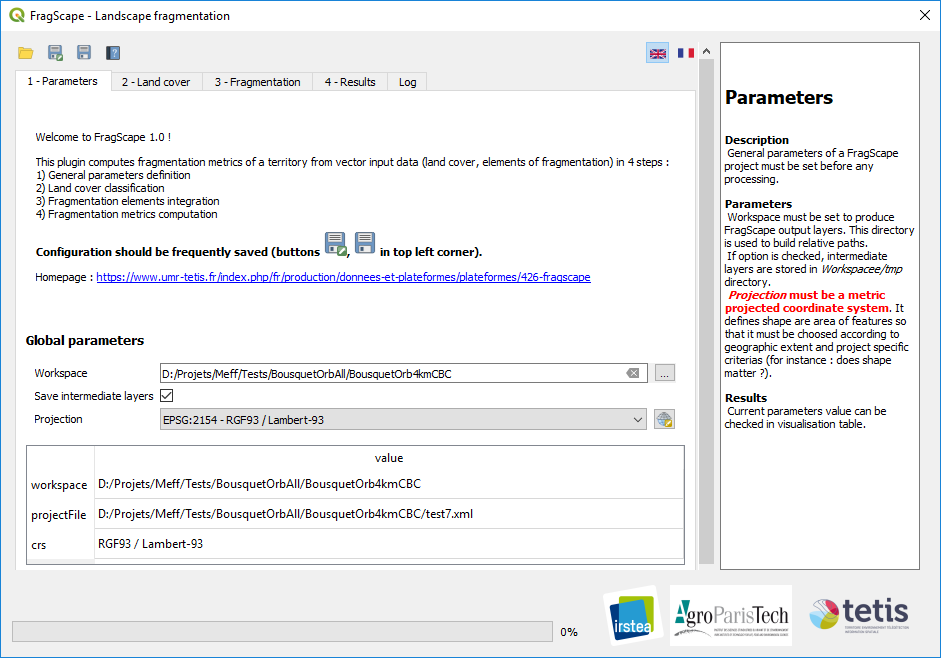
\includegraphics[scale=0.7]{pictures/paramsTab.png}
    \caption{\tool\ v1.0 Graphical User Interface}
    \label{fig:paramsTab}
    %\source{\tool\ v1.0}
\end{figure}

\pagebreak

\section{Steps}

\tool\ defines a 4 step procedure from raw data to computed metrics.

\subsection{Parameters}

First step is to define global parameters used for current \tool\ project.

\texttt{Workspace} must be set before any processing as it defines \tool\ outputs path. Output file of each step is stored in \textit{Workspace/outputs}. Be careful when setting workspace as existing file can be overriden.

If option \texttt{Save intermediate layers} is checked, intermediate layers are stored in \textit{Workspace/tmp}. Otherwise, they are stored in \qgis\ \textit{processing} temporary directory (path is displayed in log when a layer is created).

\texttt{Projection} is a projected metric coordinate reference system that must be set according to data geographic extent. It defines entities shape and area. 

\pagebreak

\subsection{Land cover}

Second step is to select target features from land cover layer.

To do so:
\begin{enumerate}
    \item Select land cover layer (\texttt{Input layer} parameter).
    \item If needed, clip \texttt{Input layer} by checking \texttt{Clip input data} and selecting \texttt{Clip layer}.
    \item Choose \texttt{Selection mode}.
    \item Choose selection criteria (fields or expression).
    \item Click on \texttt{Launch selection} button.
\end{enumerate}

In \texttt{By field values} mode, selection is performed this way:
\begin{itemize}
    \item Choose \texttt{Selection field}, e.g. the field containing land cover classes identifier (such as \textit{CODE\_2012} for Corine Land Cover 2012 data).
    \item User can choose a \texttt{Description field} that contains land cover classes description. This step is optional.
    \item Click on \texttt{Show field values} button.
    \item Select target classes in \texttt{toSelect} column of table.
\end{itemize}

In \texttt{By expression} mode, selection is performed by specifying a boolean expression. Every feature verifying this expression is selected. If no expression is specified, all features ares selected.

Figure \ref{fig:landuseTab} shows an example of land cover selection interface.

\begin{figure}[h!]
    \centering
    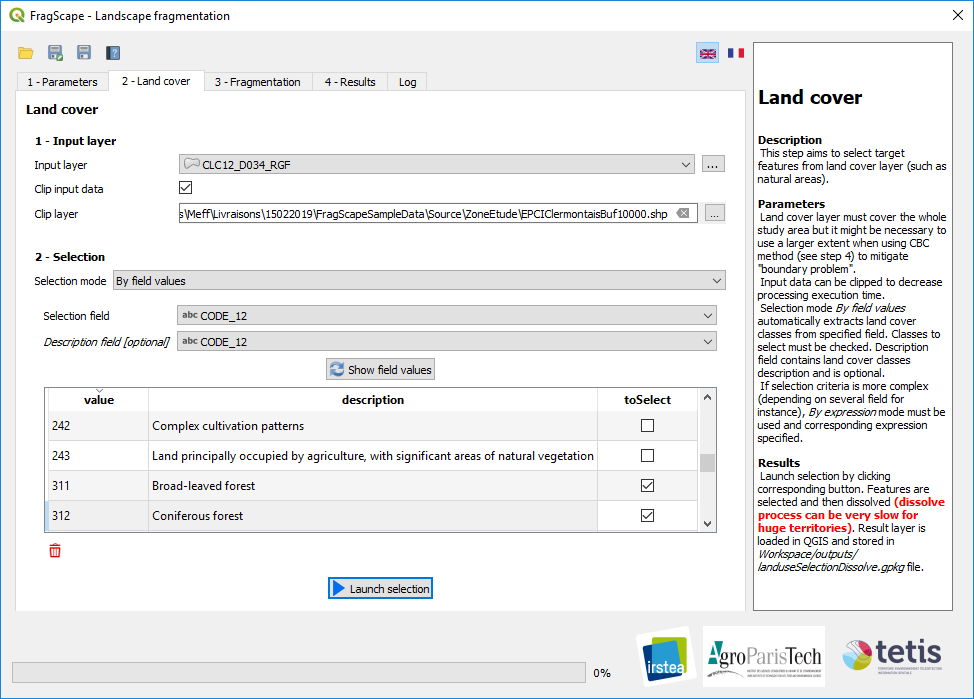
\includegraphics[scale=0.7]{pictures/landuseTabEn.png}
    \caption{\tool\ v1.0 land cover tab}
    \label{fig:landuseTab}
    %\source{\tool\ v1.0}
\end{figure}

\subsection{Fragmentation}

Third step is to select elements of fragmentation.

For each kind of fragmentation, user should:
\begin{enumerate}
    \item Select \texttt{Input layer} that contains fragmentation data ($roads.gpkg$ for instance)
    \item If needed, clip \texttt{Input layer} by checking \texttt{Clip input data} and selecting \texttt{Clip layer}.
    \item Specify selection \texttt{Expression} if needed. Features verifying this expression are selected. All features are selected if expression is empty. Expression must be boolean and built with \includesvg{pictures/mIconExpression.svg} widget.
    \item Specify \texttt{Buffer} expression. Mandatory for line and point data. Expression must be a number. Buffer expression can be variable and built through \includesvg{pictures/mIconExpression.svg} widget.
    \item Specify \texttt{Identifier} string for this kind of fragmentation. Such identifier must be unique in project.
    \item Click on \texttt{Save selection} button. Specified selection of fragmentation data appears as a new line in visualisation table.
\end{enumerate}

Once all kinds of fragmentation selected, click on \texttt{Apply fragmentation} button. For each selection, data is selected and specified buffer is applied. Buffered layers are merged to produce a layer with all fragmentation data. This layer is used to process difference with land cover layer (overlaying geometries being removed). Finally, difference layer is cast to single geometry.

Resulting layer is loaded in QGIS and stored in $Workspace/outputs/landuseFragmSingleGeom.gpkg$.

\begin{figure}[h!]
    \centering
    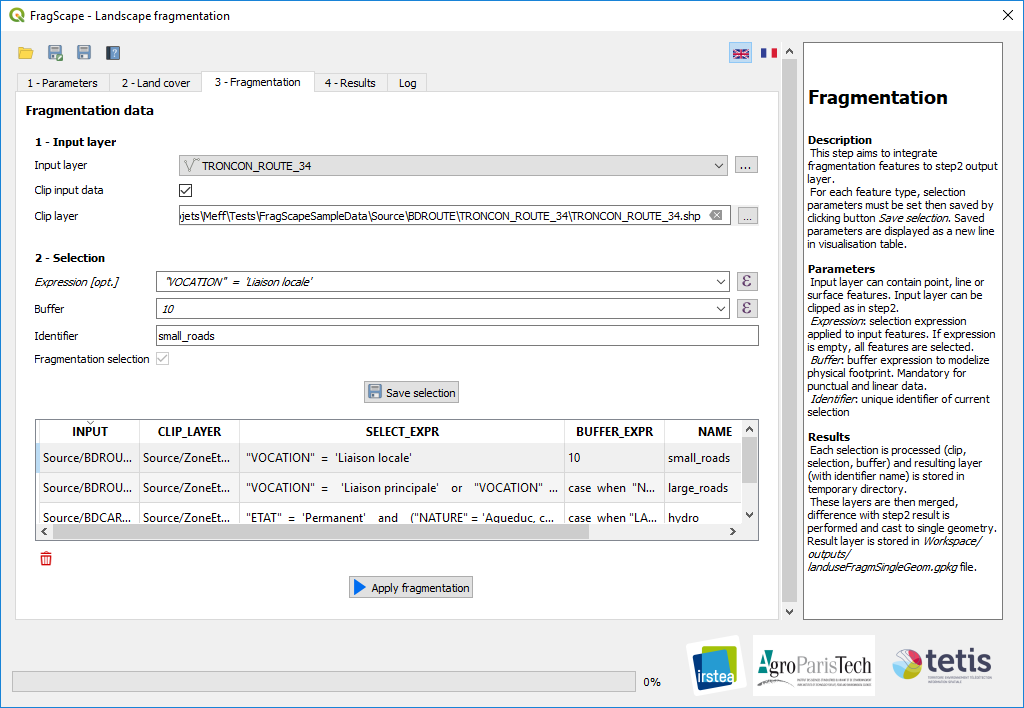
\includegraphics[scale=0.7]{pictures/fragmTabEn.png}
    \caption{\tool\ v1.0 fragmentation tab}
    \label{fig:fragmTab}
    %\source{\tool\ v1.0}
\end{figure}

\subsection{Results}

Fourth step is to compute fragmentation metrics.

To do so:
\begin{itemize}
    \item If needed, \texttt{Filter patches} by specifying a boolean expression (based on area for instance)
    \item Specify \texttt{Reporting layer}. Metrics are computed for each feature of reporting layer. To compute metrics for an entire region, specify a layer with a single feature.
    \item Select \texttt{Cut method} (see section \ref{sec:cbc})
    \item Specify \texttt{Output layer}. If not specified, a memory layer is created.
    \item Specify \texttt{Unit of area}: square meters to square kilometers.
    \item Click on \texttt{Compute metrics} button.
\end{itemize}

\begin{figure}[h!]
    \centering
    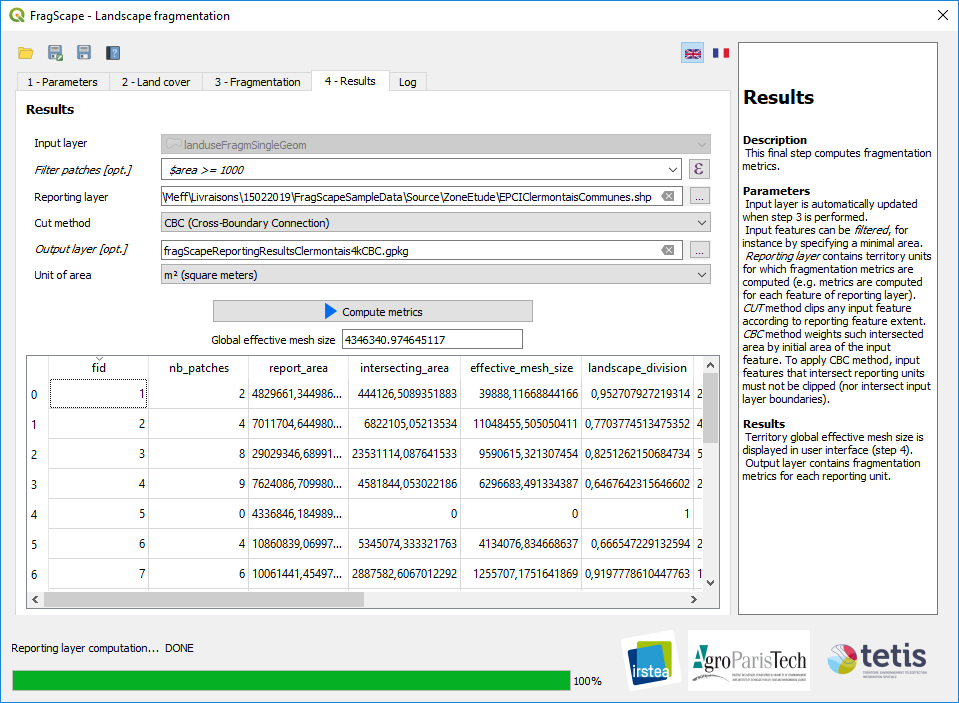
\includegraphics[scale=0.7]{pictures/resultsTabEn.png}
    \caption{\tool\ v1.0 fragmentation tab}
    \label{fig:resultsTab}
    %\source{\tool\ v1.0}
\end{figure}


Figure \ref{fig:resultsTab} shows results step interface.
Once metrics are computed, output layer attributes are loaded in visualisation table and global \meff\ is displayed.
Output layer contains a field for each metrics defined in section \ref{sec:metrics}, plus new ones :
\begin{itemize}
    \item \texttt{nb\_patches}: number of patches
    \item \texttt{report\_area}: area of the reporting unit
    \item \texttt{intersecting\_area}: intersection area of patches and reporting unit
    \item \texttt{layer/path}: temporary layer containing initial reporting unit
\end{itemize}

\pagebreak

\section{Example}

This section illustrates \tool\ use case with provided sample data (subdirectory \href{https://github.com/MathieuChailloux/FragScape/tree/master/sample_data/EPCI_Clermontais_2012}{\texttt{sample\_data}} in \tool\ plugin directory).

\begin{figure}[h!]
\centering
   \begin{subfigure}[b]{.48\textwidth}
      \includegraphics[width=\textwidth]{pictures/landuseInput.png}
      %\includegraphics[width=\textwidth]{pictures/CBC/landuseInput.png}
      \caption{Input data}
   \end{subfigure}
   \begin{subfigure}[b]{.48\textwidth}
      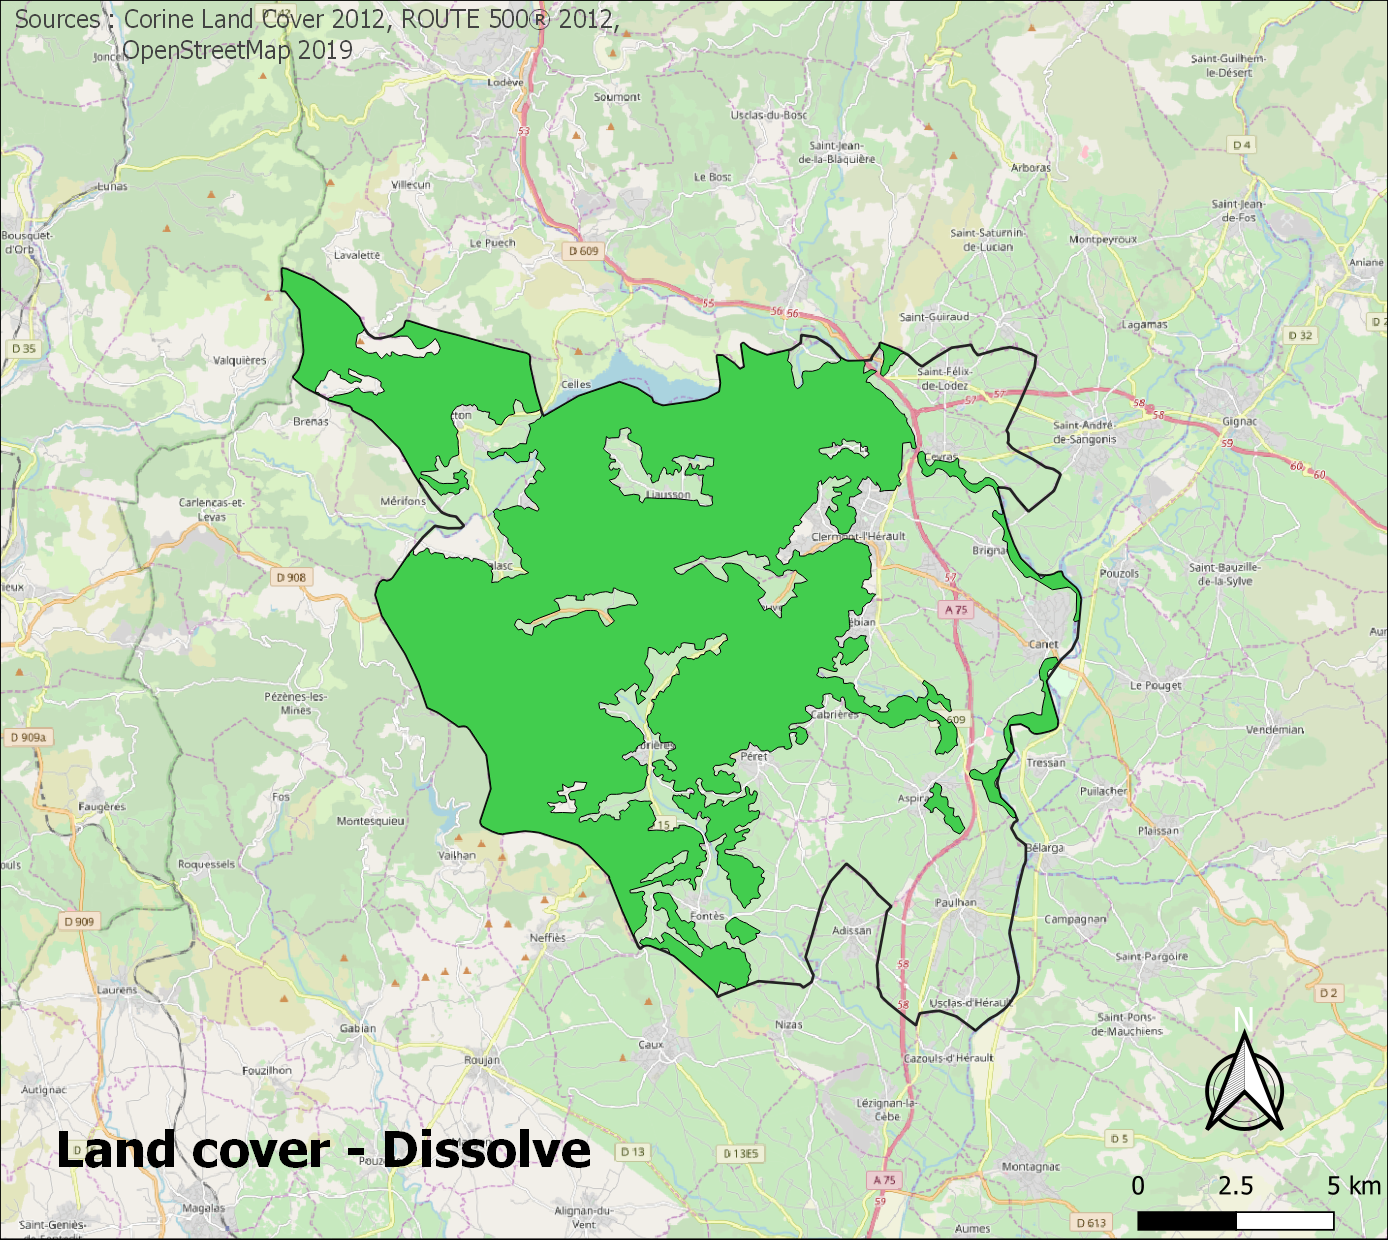
\includegraphics[width=\textwidth]{pictures/landuseDissolve.png}
      %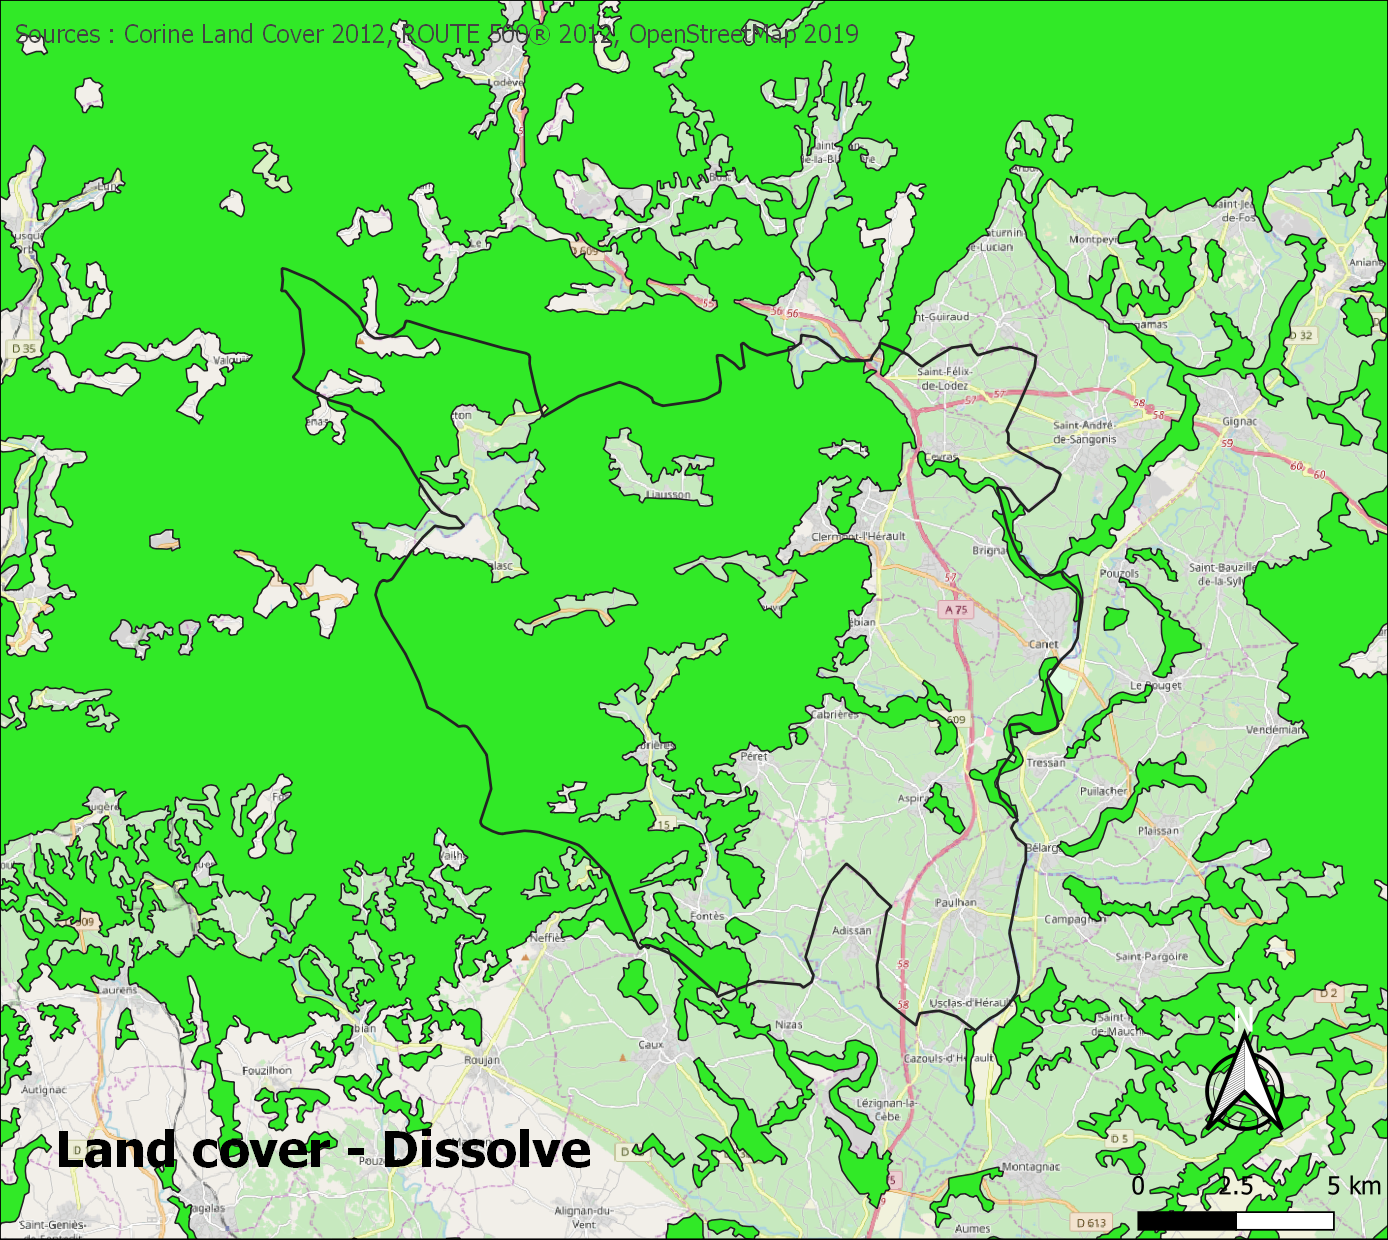
\includegraphics[width=\textwidth]{pictures/CBC/cbcLanduseDissolve.png}
      \caption{Step2}
   \end{subfigure}
   \begin{subfigure}[b]{.48\textwidth}
      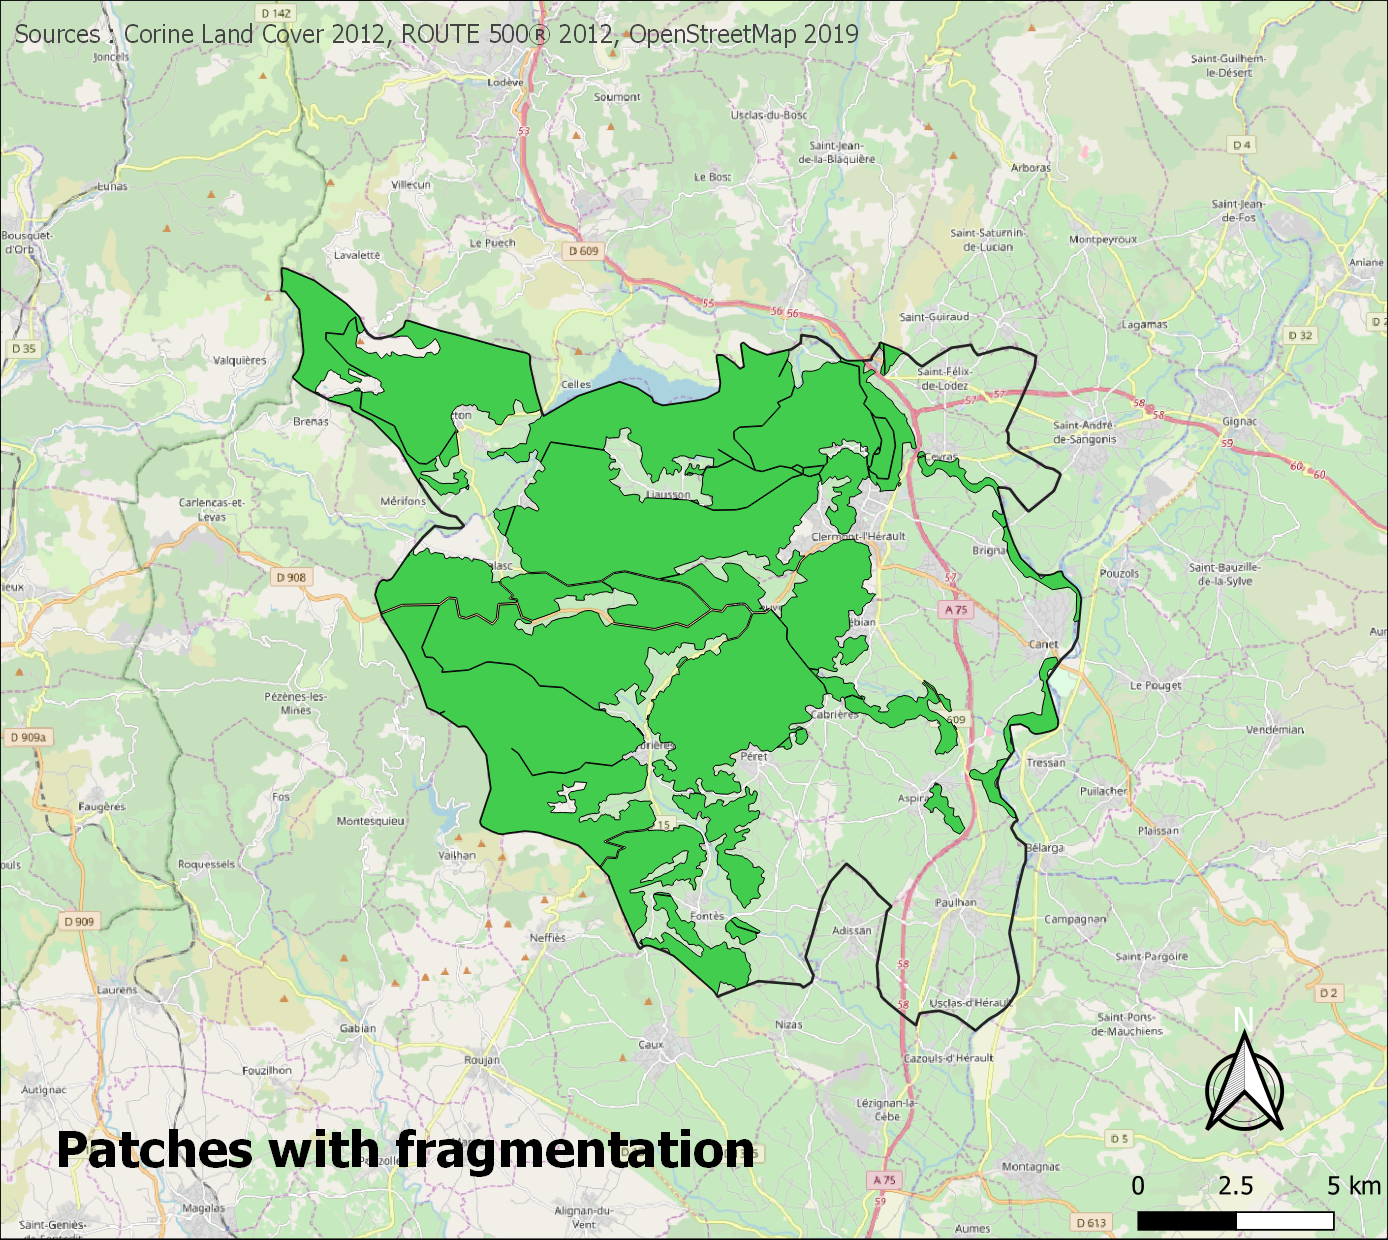
\includegraphics[width=\textwidth]{pictures/fragmPatches.png}
      %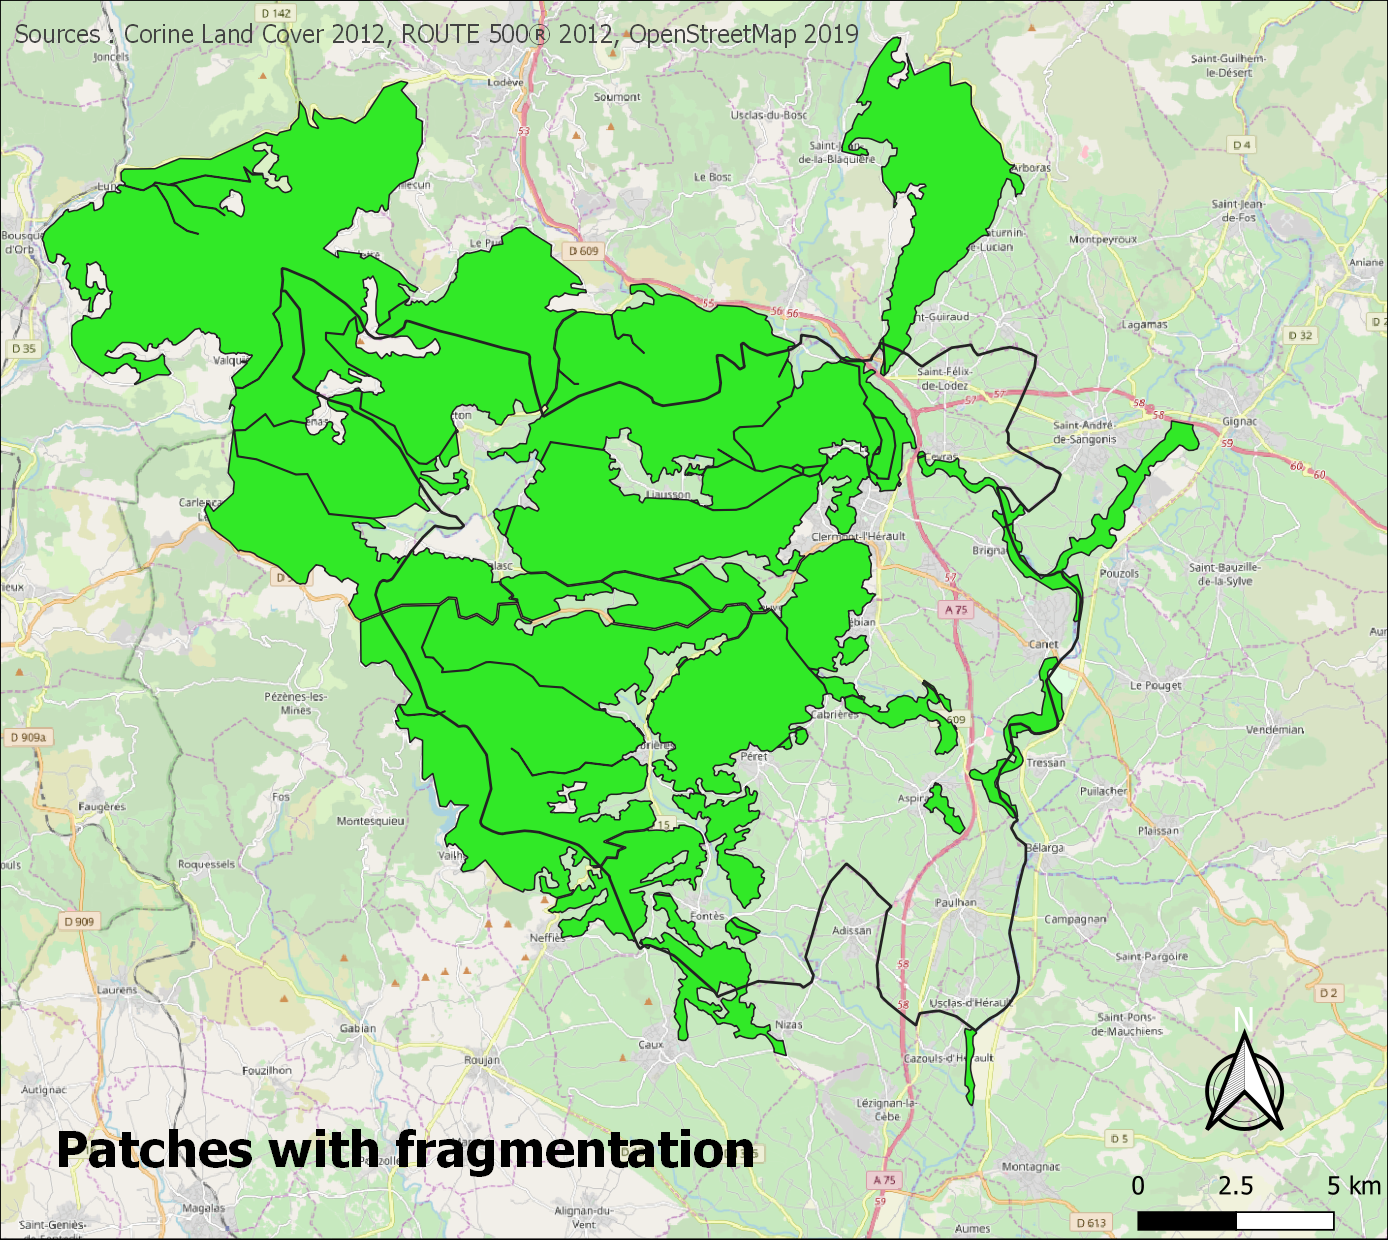
\includegraphics[width=\textwidth]{pictures/CBC/cbcFragmPatches.png}
      \caption{Step 3}
   \end{subfigure}
   \begin{subfigure}[b]{.48\textwidth}
      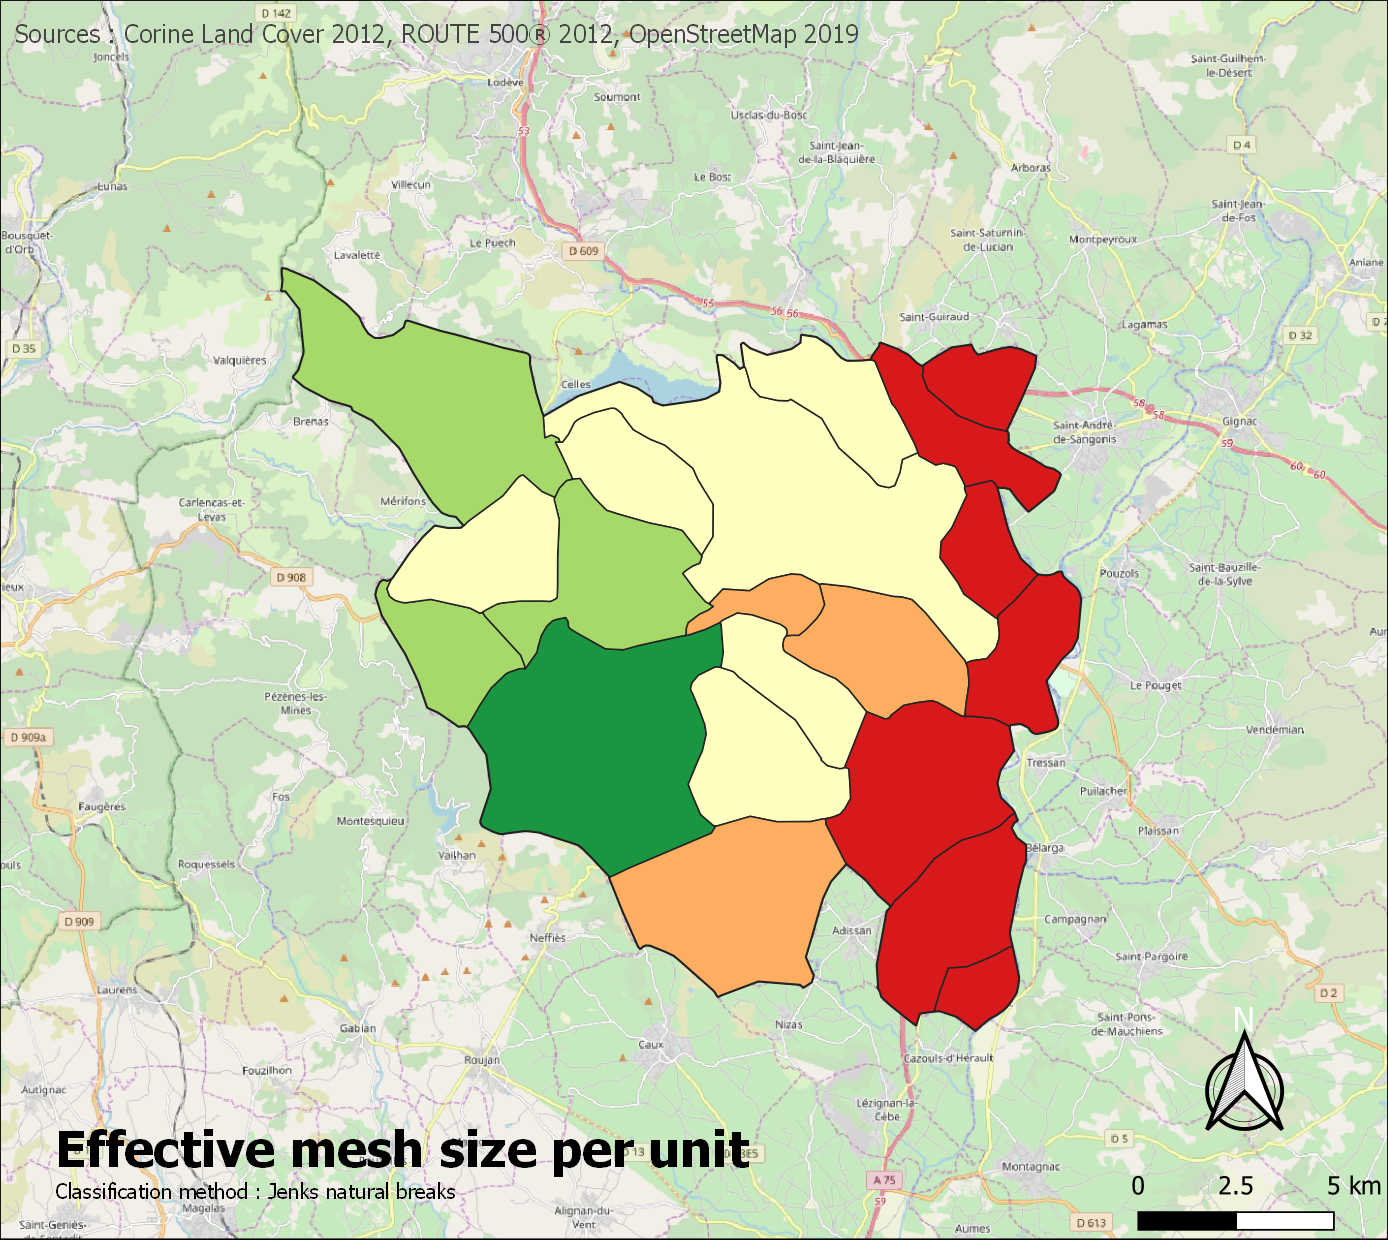
\includegraphics[width=\textwidth]{pictures/results.png}
      %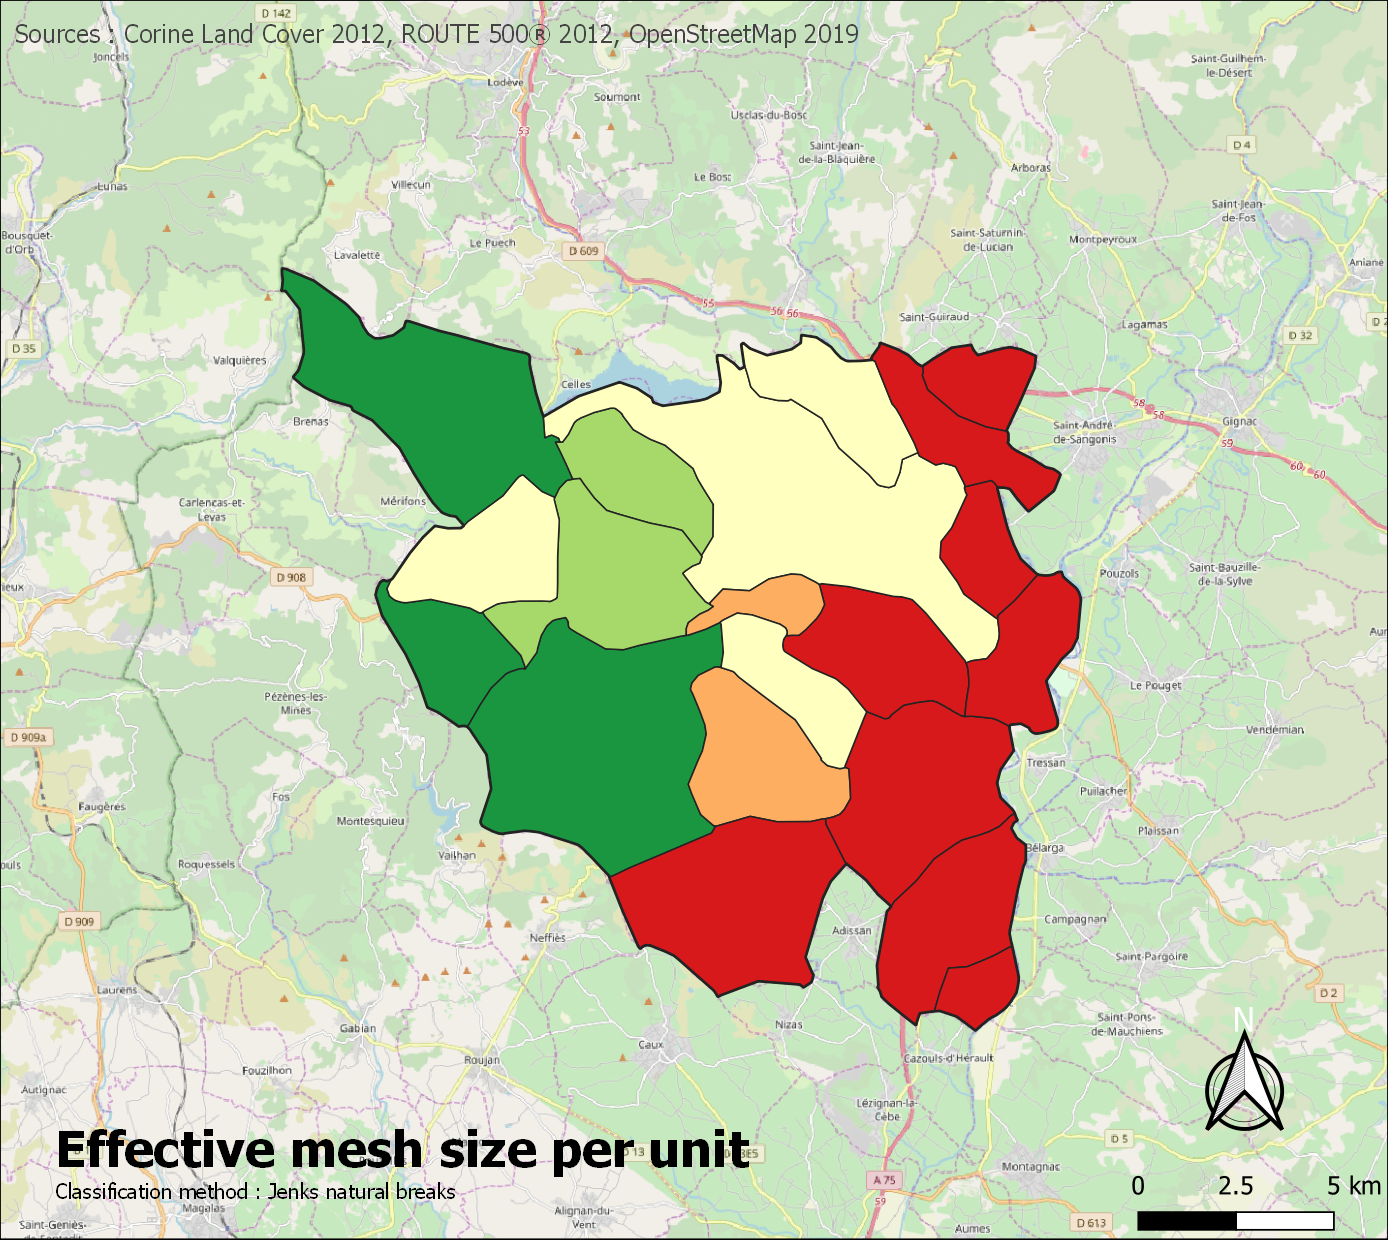
\includegraphics[width=\textwidth]{pictures/CBC/cbcResults.png}
      \caption{Step 4}
   \end{subfigure}
   \caption{\tool\ use case : from raw data to effective mesh size}
   \label{fig:usecase}
\end{figure}

Figure \ref{fig:usecase} shows input data and each step result.

To reproduce results:
\begin{itemize}
    \item Copy \texttt{sample\_data} to a local directory
    \item Open \tool
    \item Set workspace to \texttt{sample\_data/CUT}
    \item Open configuration file \texttt{EPCI\_Clermontais\_2012\_CUT.xml} from \ \includesvg[scale=0.6]{pictures/mActionFileOpen.svg} button
    \item Check that configuration has been correcty loaded
    \item Run steps 2 to 4
\end{itemize}

%Legends are not automatically generated.



%\animategraphics[autoplay,loop,width=\textwidth,controls,scale=0.5]{1}{pictures/Image_}{1}{4}

\section{To go further...}

\subsection{Execution time}

Execution time depends on region extent and \tool\ configuration. Longest steps are usually geometries dissolve at step 2 and difference at step 3.

A complete benchmark is currently being performed by applying simple and complex configurations to regions of different scales (french department Hérault, old region Languedoc-Roussillon, new region Occitanie, and finally whole France).

Some examples of execution time (but performed with different configuration and versions of \tool, these are \textbf{indicative values}):

\begin{center}
\begin{tabular}{|c|ccc|}
    \hline
    Test case & Step 1 & Step 2 & Step 3 \\
    \hline
    Languedoc-Roussillon & 40s & 137s & 72s \\
    Occitanie & 5mn25s & 11mn25s & 1mn54s \\
    France & 122h & 19h & 5h \\
    \hline
\end{tabular}
\end{center}


\subsection{Configuration file}

Configuration is saved as an XML file and thus can be opened in a text editor. Figure \ref{fig:configFile} shows the begining of configuration file \texttt{sample\_data/ECPI\_Clermontais\_2012/CBC/ECPI\_Clermontais\_2012\_CBC.xml}

\begin{figure}[h!]
    \centering
    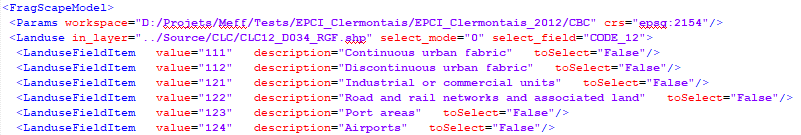
\includegraphics[scale=0.8]{pictures/configFile.png}
    \caption{Example of a configuration file}
    \label{fig:configFile}
    %\source{\tool\ v1.0}
\end{figure}

In \textit{Landuse} tag, one can see attributes such as \textit{in\_layer} (input layer), \textit{select\_mode} ($0$ meaning selection mode \texttt{By field values}) and \textit{select\_field} (selection field of input layer is \textit{CODE\_12}).
For each loaded field value, a \textit{LanduseFieldItem} tag exists and contains same attributes as in \tool\ (\textit{value}, \textit{description}, \textit{toSelect}).

Such file can be manually edited if needs be. For instance if relative paths must be changed for a new project (\texttt{../Source} becoming \texttt{../../Source}), updating it in \tool\ tables or creating a new project can be avoided by editing new paths in configuration file and then reloading it.

%\subsection{Algorithms}

\pagebreak

\subsection{Algorithms}
\label{sec:algs}

\begin{minipage}[c]{.46\linewidth}
\tool\ steps are implemented as \qgis\ $processing$ algorithms. As shown in figure \ref{fig:algs}, five algorithms are provided:
\end{minipage} \hfill
\begin{minipage}[c]{.5\linewidth}
    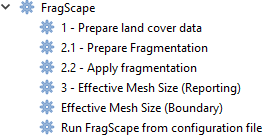
\includegraphics[scale=1]{pictures/algs.png}
    \captionof{figure}{\tool\ algorithms}
    \label{fig:algs}
\end{minipage}


\begin{enumerate}
    \item \texttt{1 - Prepare land cover data}: performs selection and geometries dissolve as in step 2 except that selection expression must be directly provided (in \tool, expression can be built from checked field values)
    \item \texttt{2.1 - Prepare fragmentation data}: performs selection, and applies a buffer to a layer containing fragmentation elements to represent its physical footprint. This algorithm is called for each line/kind of fragmentation in step 3.
    \item \texttt{2.2 - Apply fragmentation}: builds a layer of patches from a land cover layer and fragmentation layers. Fragmentation layers are merged, overlaying geometries with land cover data are removed and remaining ones are cast to single geometry type. This algorithm is called at the end of step 3.
    \item \texttt{3 - Effective mesh size (Reporting)}: computes landscape metrics described in section \ref{sec:metrics} from a layer of patches for each entity of a reporting layer according to specified method (see section \ref{sec:cbc}). This algorithm is called at step 4 to produce output layer.
    \item \texttt{Effective mesh size (Boundary)}: computes landscape metrics as previous algorithm except that reporting layer must contain only one feature. This algorithm is called at step 4 for each reporting unit and to compute global effective mesh size.
    \item \texttt{Run \tool\ from configuration file}: executes \tool\ processing chain from a \tool\ configuration file. This algorithm can be useful to reproduce results from an existing configuration, launch processing tasks in background or to executes all steps at once.  
\end{enumerate}




\section{FAQ}

\begin{itemize}
\item \textbf{Fields are not loaded in field/expression widget \includesvg{pictures/mIconExpression.svg}, why ?} If they don't appear, it is because associated layer is not loaded even if its path is displayed in combo box. Select another layer and then re-select initial layer.

\item \textbf{Which method should I use, CUT or CBC ?} CBC method has been designed to address boundary problem and then should be used. CUT method is available to allow comparison with already computed results, or in case boundaries are not a problem.

\item \textbf{Elements of fragmentation are already included in my land cover layer, should I run step 3 ?} In \tool\ 1.0, input layer of step 3 and 4 cannot be specified and must be generated by \tool. In case fragmentation elements are already included in land cover data, launch step 3 without any fragmentation element. 

\item \textbf{Can I apply \tool\ processing to layer not produced by \tool\ ?} To apply \tool\ specific processing to specific data, one can use \tool\ algorithms described in section \ref{sec:algs}.

\end{itemize}

\frameboxbegin{Good practices}
\begin{itemize}
    \item Do not use spaces and special characters in file names.
    \item Do not use special characters in field values.
    \item Save \tool\ configuration at each step.
    \item Check each step result.
    \item If a problem occurs, save configuration, exit \tool\, relaunch \tool\ and re-open saved configuration. If problem still occurs, exit and relaunch QGIS. If problem still occurs, contact support team.
\end{itemize}
\frameboxend

\subsection*{Error messages}

\begin{itemize}
    \item \textbf{\color{red}Layer XXX is already loaded in QGIS, please remove it.} \tool\  cannot delete file if it is already loaded. Just remove it from QGIS project and relaunch \tool\ processing.
    \item \textbf{\color{red}The process cannot access the file because it is being used by another process: XXX.} Check that XXX file is not used by another process. If not, save configuration, save QGIS project, exit QGIS, relaunch QGIS, relaunch \tool, re-open configuration and relaunch \tool\ processing. This is a known bug when relaunching step 3 after step 4.
\end{itemize}

\textbf{\color{red}}



%\subsubsection*{}

\addcontentsline{toc}{section}{Bibliography}
\printbibliography

\end{document}
